\documentclass[aps,prd,preprint]{revtex4}
%\documentclass[aps,prd,twocolumn,twoside,floatfix]{revtex4}

\usepackage{pioneer}
\def\theAuthor{Tony Lu}
\def\theYear{2016}
\usepackage{graphicx}
\usepackage{bibentry}
\usepackage{csquotes}
\usepackage{listings}

\begin{document}
\pagestyle{pioneer}
\date{July 8, 2016}
\preprint{}
\title{Undecided Title}
\author{Tony Lu}

\begin{abstract}
The detection of gravitational was a piece of flash-news. In some sense, it was quite coincident that a detection was made almost immediately after the testing launch of Advanced Laser Interferometer Gravitational Wave Observatory. I took the waveform signal of the event GW150914 to make injections on data from LIGO's S6 run and recovered them. Overall, none of signal-to-noise ratio values I recovered was high enough to claim a detection. In the later portion of S6 where noise was less loud, the signal could be identified as a candidate event. However, I also noticed that if the distance from the system is closer, LIGO at S6 would have the potential to make the detection.
\end{abstract}
\maketitle



\section{The Main Questions}
One of the deciding factors that made the detection of elusive gravitational waves possible is the sensitivity of the equipment. Over the LIGO's S5 \cite{S5}, S6 \cite{S6} and O1 \cite{O1} (which the scientists used to refer to as S7) runs, the sensitivity was improved significantly each time, with effective attenuation of noise.
\par At some degree, the detection seemed very much like a coincidence, for no detection in the past two decades was made until the one made within just one week after the testing launch of Advanced LIGO \cite{timeline}. So here's a question: was LIGO at any early stage sensitive enough to make this detection? Was the detection of GW150914 a coincidence?
%============================================================


\section{Background Information}
More than a century ago Albert Einstein's General Theory of Relativity stated that we live in a four dimensional world\textemdash space-time (three dimensions for space and one for time). Masses cause distortions in spac-time, which accounts for the phenomenon of gravity. And the theory predicts that changing mass distribution will generally produce ripples in space-time, which is another prediction from him\textemdash gravitational waves. \cite{relativity1,relativity2} For decades, scientists have been struggling to detect gravitational waves from outer space. They upgraded their detectors over and over again, just in order to catch the whisper from distant celestial bodies. Fortunately, on September 14, 2015, the LIGO detectors successfully recorded the signals from two colliding black holes, which was the first direct detection of gravitational waves ever, a remarkable one. \cite{O1} It is labeled GW150914.
\par This section aims to provide background information about LIGO and gravitational waves. The section ...
%---------------------------------------------------------------------------------------

\subsection{Introduction to Gravitational Waves}
Einstein found that his linearized weak-field equations have wave solutions. \cite{O1} These transverse waves are \emph{ripples} in the \emph{fabric} of space-time, caused by some strong and catastrophic happenings in the universe.
\par According to Einstein's calculations, gravitational waves are generated by objects accelerating with asymmetric motion. To be more precise, gravitational waves require changing quadrupole mass distribution. Generally, the amount of gravitational waves given off is positively correlated to the system's mass and its speed of motion. Changes in space-time produced by a moving mass are not felt in the distance at once, but they propagate at the speed of light. \cite{SBackground}
\par Gravitational waves are transverse waves, the same as electromagnetic waves, but they are waves of changes in tensors (quadrupole distortions of space-time) which result in expansions and contractions in lengths in certain directions. Unlike the horizontal and vertical polarizations of electromagnetic waves, the those of gravitational waves are \enquote{plus} and \enquote{cross}. However, gravitational waves do share lots of similarities with electromagnetic waves. They have frequencies and wavelengths, whose relationship is given by: $\lambda f=c$, where $\lambda$ is the wavelength, $f$ is the frequency, and $c$ is the speed of light. They are able to carry energy, momentum, and angular momentum away from the source. \cite{SBackground} The strain amplitude can be derived from Einstein's quadrupole formula, and it's inversely proportional to the distance from the mass center. \cite{relativity2} It can also be measured by ratio of the change in length to the original length $h=\frac{\Delta L}{L}$. 
\begin{figure}
	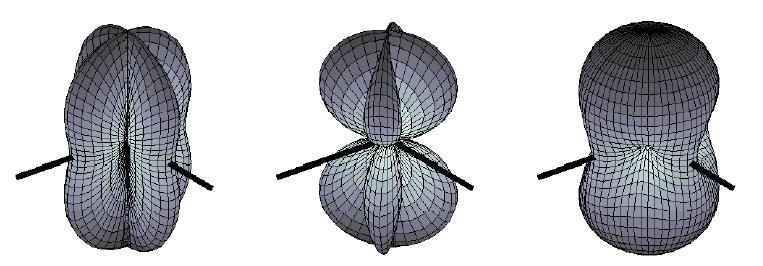
\includegraphics{G-wave_polarizations}
	\caption{The pattern on the left is for plus polarization, the middle pattern is for cross polarization, and the right-most one is for unpolarized waves. The black lines are the arms of LIGO detectors, which will be addressed in \ref{sec:LIGO}. Source: \cite{S6Run}}
\end{figure}
\par Gravitational waves have various sources, but there are mainly four catagories: stochastic backgroud, bursts from gravitational collapse, pulsars, and binary systems. Binary systems refer to those that consist of two bodies rotating aroung each other. Whether or not the two stars collide, gravitaional waves will be generated. The detection made on September 14, 2015 is the collision of two black holes, which is named compact binary coalescence\textemdash \enquote{chirp}. \cite{O1} More details are given by \cite{SBackground} in section 3.
%---------------------------------------------------------------------------------------

\subsection{Introduction to LIGO \label{sec:LIGO}}
Distortions in space-time is almost impossible to measure directly, for if you use a meter stick, the meter stick itself will expand and contract with changing space-time. Fortunately, lights remain the same speed despite any deformation of space-time, which sets the basis for the LIGO detectors. \cite{CaltechLIGO}
\par The detectors of LIGO\textemdash Michelson Interferometer\textemdash was invented by Albert Abraham Michelson, first used in the famous Michelson-Morley experiment \cite{Michelson-Morley}. Its function is for optical interferometry. With a beam splitter, a light source is split into the two arms, and each of the new beam is reflected back and combined again. The result of such combination leads to optical interference—either constructive or destructive—depending on the changes in length of the arms. Therefore, the photo detector could sense the variation in the arms’ length. \cite{CaltechLIGO}
\par The interferometer in LIGO consists of two vacuum arms of equal length\textemdash 4 kilometers long, which form an L shape. There is a laser light source and a photodetector at about the corner of the L, and a beam splitter at the corner. At each end and in the middle of the arms freely hanged four mirrors which reflects the laser beam, and the two beams are combined into one at the beam splitter. Those mirrors in the middle are used to increase the distance light beams travel, and as a result, the actual effective length is increased from 4km to 1120 km, greatly enhancing LIGO's sensitivity. If the arm length changed, the two light beams which were originally in phase would be out of phase, creating destructive interference which allows the photodetector to sense the infinitesimal change in length of the arms. \cite{CaltechLIGO, MitLIGO}
\begin{figure}
	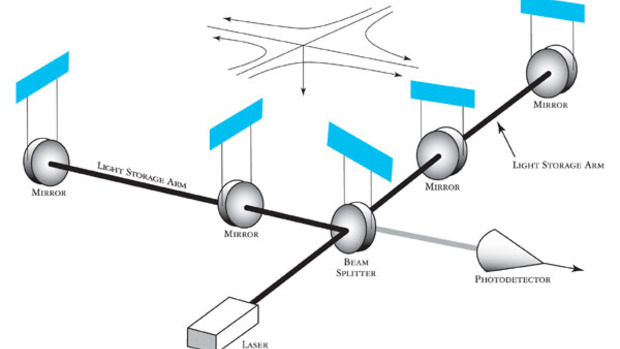
\includegraphics{basic_ifo_diagram}
	\caption{Basic schematic of LIGO's interferometers with an incoming gravitational wave depicted as arriving from directly above the detector. Source: \cite{CaltechLIGO}}
\end{figure}
\par Moreover, the two LIGOs in the US are located in Livingston Parish , Louisiana and Hanford , Washington. Both are L-shaped and of the same size--their arms are all 4km long. The two Ls are in different directions, and they are separated by 3030.3 kilometers  on land, which means the planes these observatories are on have a dihedral angle of 27.3 degrees. \footnote{By Google Earth} Therefore, it's guaranteed that gravitational waves from any directions can be detected, given enough sensitivity.
\par A brief history of LIGO is given by \cite{BHLIGO}. A more technically and quantatatively detailed description of LIGO is given by \cite{S6Run}.
%---------------------------------------------------------------------------------------

\subsection{Sensitivity of the Detectors}
Similar to any real physics experiment, the LIGO detectors face various disturbance from the environment. Considering the small amplitudes of gravitational waves, we see that sensitivity become decisive. At the very beginning of the construction, the interference of the noises are so high that it was even impossible for the detectors to collect data clean enough to analyze. But the quality of data collected has been significantly improved over the several stages of LIGO. The datasets of its S5 (2005-2007), S6 (2009-2010), and O1 (2015-present) are available online. \cite{TLdata} Among all these sensitivity-limiting factors are primarily: seismic noise (at relatively low frequencies), thermal noise (at mid frequencies), shot noise (at high frequencies), and the problems with the lasers and electronics. Some more specific details, including solutions, are given by \cite{Noise, thermal, seismic}
\par The problems related to sensitivity are curious to investigate. My research is closely related to sensitivity.
%---------------------------------------------------------------------------------------

\subsection{Injections}
In short, injections are used to test if the detectors are working well. There are two types of injections: hardware injections and software injections. The first type is made by manually changing the position of the mirrors in the interferometer. The second type is achieved by adding signal directly into the data flow. Moreover, there were those called \enquote{blind injections}, when few scientists know it was an injection while the majority were convinced that it really was a detection. One of the famous events was the one back in 2010, which was reported in \cite{blindInj}.
%---------------------------------------------------------------------------------------

\subsection{The GPS Time}
GPS time is a system to keep track of time. It is the total number of seconds from 00:00:00 January 6, 1980 UTC.
%=========================================================


\section{Research Methodology Description}
This section aims to provide a description of the overall methodology to obtain the raw data for further analysis of my investigation.

\subsection{Data Files}
\subsubsection{Event Waveform}
The strain data of the GW150914 event I used is from the LOSC site. Specifically, it's form the waveform.txt file from the \enquote{Download the Data} section in \cite{GWTutorial}. This strain data was later used as the signal for my self-made injection.
\subsubsection{Template for Recovery}
As for the template for injection recovery (see: \ref{sec:Recovery}), it's different from the waveform. It is included in the zip file of another tutorial. \cite{GWTutorial2} The complex template contains two waveforms, one of which is used as the real part and the other as the imaginary part. Moreover, as pointed out in the \enquote{Waveform Template} of this tutorial, the templates are not 100\% the same as what the scientists actually used. Many subtleties are skipped, for example. But the quality of the templates online is good enough for my investigation.
\subsubsection{Background\textemdash Noise \label{sec:dataFile}}
The background strain data of my injections were selected from a number of data files from LIGO's S6 run, from GPS time 931035615 to 971622015. The S6 data archive is on this page \cite{S6Data}. Because of the probable fluctuation in the power of the background noise over the entire S6 run, I chose 10 different and relatively evenly dispersed data files, each starting at GPS time 931127296 (0.226\%), 934846464 (9.39\%), 941707264 (26.3\%), 941785088 (26.5\%), 947154944 (39.7\%), 952623104 (53.2\%), 959344640 (69.8\%), 963629056 (80.3\%), 967442432 (89.7\%), and 971407360 (99.5\%), all lasting for 4096 seconds.
%---------------------------------------------------------------------------------------

\subsection{Data Quality Vetoes}
The background quality is critical. A piece of low-quality data could result in a misleading outcome. Furthermore, that kind of datafiles would be vetoed by the scientists. Even if there really were an event, it would not be searched and detected. And it becomes useless for me do investigate on such a data file.
\par In general, I needed to assure that the background I was injecting on has its proper data quality flags on. Because the event of GW150914 is a compact binary coalescence system \cite{O1} and the mass is big enough to be catagorized as \enquote{high mass} \cite{S6himass}, the flag of \enquote{CBCHIGH\textunderscore CAT4} should be on. Besides, there should not be any other injections which would affect my recovery, so the flag of \enquote{HW} should be off. \cite{S6DQ}
%---------------------------------------------------------------------------------------
 
\subsection{Making the Injections}
The injections were made by simply superposing the waveform on to the background signal. Ten injections were made to each of the ten data files at randomly selected points. The data quality flags for compact binary coalescence hardware injections were modified as well. In addition to the original strain, I amplified the waveform signal by a factor of 2, 3, 5, 8, 12, 20, 40, and zero, and thus did 8 more groups. In total, that was 800 injections. The script for making these injections is attached in \ref{sec:Appendix1}.
%---------------------------------------------------------------------------------------

\subsection{Injection Recovery \label{sec:Recovery}}
To recover the injection, I computed the SNR of each injection using matched filter. The processing was essentially the same as that in \cite{GWTutorial}. The scripts for recovery are attached in \ref{sec:Appendix2}.
%---------------------------------------------------------------------------------------

\subsection{Software Support}
The main software for analysis is Python 2.7.11, Anaconda 2 (iPython), and Excel 2013 with excel2latex macro.
%---------------------------------------------------------------------------------------

\subsection{Some Relevant Statistical Concepts and Algorithms}
\subsubsection{Signal-to-noise Ratio\textemdash SNR}
Signal-to-noise ratio (SNR) \cite{SNR} indicates the relative power of the signal to the background noise. The value is a positive figure greater or equal to one.
\subsubsection{Matched Filter}
Matched filter \cite{findChirp} is an algorithm that computes the SNR.
\subsubsection{Root Mean Square\textemdash RMS}
Root mean square is calculated by taking the square root of mean of the squared values of all the samples: $x_{RMS} = \sqrt{\frac{x_1^2 + x_2^2 + ... + x_n^2}{n}}$ \cite{RMS}
\subsubsection{Linear Regression}
Linear Regression is an approach to model the relationship between a dependent variable and an independent variable. The result is that the depend variable is a linear function of the independent one: $y = ax+b$ \cite{regression}
\par Additionally, there is a concept called correlation coefficient. The result, $r^2$, is a measure of how well the values fit the model, therefore indicating the accuracy of the model. The closer $r^2$ is to 1, the better the values fit the model. If $r^2$ equals one, all the values lie on the model. \cite{r_squared}
%===========================================================


\section{Data Analysis}
This section presents the data analyzing process. The data files obtained in \ref{sec:dataFile} are referred to as data file number one to ten, respectively.

\subsection{Computing the RMS of Strain Data}
In this case, RMS functioned as a representation of the significance of the noise in each data file. It can be inferred from the RMSs that noise in the detectors is generally louder earlier in S6 than later in S6, which is consistent with other results coming up.
\par\#\#Insert Scatterplot Graph\#\#
%---------------------------------------------------------------------------------------

\subsection{The Mean SNR of Each Data File at Different Amplifications}
Before calculating the mean SNR of each piece of data, I manually discarded some extreme values which appeared to be anomalies. These extremities may be caused by a sudden fluctuation in the background noise, a mistake in the computation, or an injection failure. The mean SNR was simply taken by computing the average recovered SNR value of the 10 injections (except the anomolies) of each data file at each amplification.
\par The figures in Table \ref{tab:SNR} indicate that the matched filter output for background noise is generally at a level of 4 or 5. Sometimes, there may even be a spike in the SNR that reaches 6 or more. So the SNR values taken where the injection signals were not amplified (aplification equals one) are not credible, for they are mostly 6 or less. Instead of the injections, those SNRs could have been caused the spikes in the background noise. Therefore, I needed to use regression analysis to model the SNR against amplification, thus predicting the SNR where the signal was not amplified.
\begin{table}
	\caption{The average SNRs recovered from the ten data files at 8 different amplifications of the injection signal. The amplification of zero means the SNR is recovered from pure background noise. \label{tab:SNR}}
	% Table generated by Excel2LaTeX from sheet 'Sheet5'
	\begin{tabular}{c|ccccccccc}
		\hline
		\hline
		& \multicolumn{ 9}{|c}{Amplification} \\
		\hline
		File Number & 0 & 1 & 2 & 3 & 5 & 8 & 12 & 20 & 40 \\
		\hline
		1 & 4.967  & 4.963  & 8.053  & 12.886  & 21.483  & 32.060  & 49.788  & 79.564  & 148.866  \\
		
		2 & 4.864  & 4.851  & 8.947  & 13.161  & 20.177  & 35.378  & 51.638  & 74.457  & 154.196  \\
		
		3 & 6.235  & 6.184  & 7.973  & 12.590  & 20.627  & 33.050  & 49.999  & 80.095  & 150.797  \\
		
		4 & 5.587  & 5.766  & 8.664  & 14.936  & 26.684  & 40.671  & 60.653  & 94.043  & 175.344  \\
		
		5 & 4.626  & 5.096  & 10.326  & 15.288  & 25.616  & 40.149  & 61.203  & 98.755  & 175.360  \\
		
		6 & 4.613  & 6.160  & 11.861  & 18.152  & 29.805  & 46.423  & 70.410  & 116.439  & 206.434  \\
		
		7 & 5.100  & 8.176  & 12.717  & 18.842  & 31.322  & 49.614  & 70.877  & 118.420  & 202.897  \\
		
		8 & 4.675  & 6.032  & 12.165  & 17.230  & 34.306  & 46.488  & 70.337  & 111.888  & 191.332  \\
		
		9 & 4.570  & 6.479  & 10.079  & 17.501  & 28.178  & 47.082  & 64.857  & 113.912  & 203.616  \\
		
		10 & 4.980  & 6.489  & 12.096  & 19.185  & 30.698  & 50.930  & 67.298  & 120.715  & 206.301  \\
		\hline
		\hline
	\end{tabular}  
\end{table}

\begin{figure}
	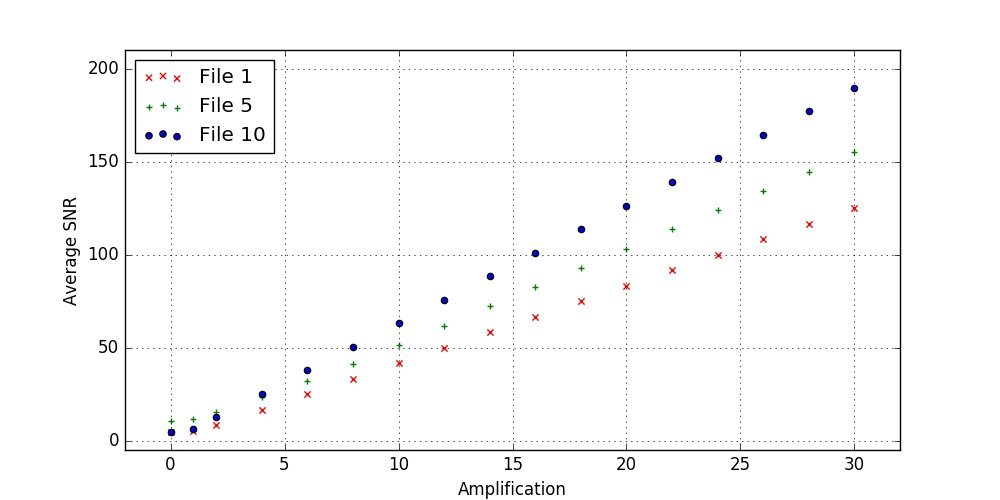
\includegraphics[width=\textwidth]{SNRs}
	\caption{something}
\end{figure}
%---------------------------------------------------------------------------------------

\subsection{Computing the Linear Regression}
First of all, I chose linear regression to be the type of my model. Due to the nature of the concept of SNR, the amplification (signal power) should be positive correlated to the output. Meanwhile, the output goes up neither exponentially nor logarithmically, but it increases at a steady rate, so linear model should be the best fit. I further specified the intercept as zero, for theoretically the output should be zero when no signal exist in the noisy background.
\par If we were to test the models, we would find that the regressions would somewhat underestimate the SNRs at low amplifications. So in reality, the SNRs should be at somewhere between the second colume of data in Table \ref{tab:SNR} and the values in \ref{tab:predict}. Nevertheless, the highest possible SNR was only around 6.5, which means the signal would be overwhelmed by the noise and unable to stand out.
\begin{table}
	\caption{Linear regression computed from the data in Table \ref{tab:SNR}, with intercept set to zero. The leftmost colume presents the predicted SNR when no amplification was made. \label{tab:predict}}
	% Table generated by Excel2LaTeX from sheet 'Sheet8'
	\begin{tabular}{crrc}
		\hline
		\hline
		File Number & Slope & R-Squared & Predicted SNR \\
		\hline
		1 & 3.812  &  & 3.812  \\
		
		2 & 3.882  &  & 3.882  \\
		
		3 & 3.854  &  & 3.854  \\
		
		4 & 4.516  &  & 4.516  \\
		
		5 & 4.559  &  & 4.559  \\
		
		6 & 5.356  &  & 5.356  \\
		
		7 & 5.330  &  & 5.330  \\
		
		8 & 5.055  &  & 5.055  \\
		
		9 & 5.250  &  & 5.250  \\
		
		10 & 5.395  &  & 5.395  \\
		\hline
		\hline
	\end{tabular}  
\end{table}
%==========================================================

\section{Conclusion}
I found that the GW150914 event would not be loud enough for LIGO at S6 run. The signal could, at best, be identified as a candidate event, but it's significance would be far from enough to claim a real detection. In short, the S6 run is not sensitive enough to make this detection. Therefore, GW150914 event was not a mere coincidence. In contrast, the successful detection was and (the future detections are) made possible by persisting in upgrading the detectors, which are really worth doing.
%==========================================================


\section{Extensions}

%==========================================================

\section{Appendix A: Python Scripts}
These are the Python scripts I used for my research.
\subsection{For Making Injections \label{sec:Appendix1}}
\lstinputlisting{inj2.py}
\subsection{For Recovery\textemdash Bulk Operation \label{sec:Appendix2}}
\lstinputlisting{go2.py}
%==========================================================


\section{Appendix B: More Data Tables}
\bibliography{Paper3,Paper1Background,Paper2Proposal}
\end{document}